\section{Routing e Sicurezza}
\subsection{Routing Statico}
Il routing statico, anche denominato come instradamento statico, è un metodo che sfrutta percorsi prefissati dall’amministratore di rete. In questa maniera si può configurare un'intera rete molto velocemente, anche se con alcuni svantaggi. Infatti, il routing statico, avendo gli indirizzi fissi nelle varie macchine della rete, non è efficiente nella risoluzione di possibili errori. 

Il grande problema, infatti, si ha nel direzionare il pacchetto nella rete, se il percorso previsto per il pacchetto ha un errore al suo interno il traffico non viene ridirezionato e attende finché il percorso non sia stato riparato o finché l'amministratore di rete non abbia definito una nuova rotta. 

Nonostante ciò, però, il routing statico è ancora molto utilizzato e permette a piccole sottoreti interconnesse di lavorare al meglio e con pochi sforzi di gestione.

\subsubsection*{Configurazione computer con IP statici}
Per assegnare degli indirizzi IP in maniera statica ai dispositivi in una rete bastano 4 step, vediamone un esempio concreto svolto su CISCO packet tracer:

\begin{enumerate}
    \item Per prima cosa aprire la finestra relativa al dispositivo in questione (in questo caso un PC)\par
    \begin{sfigure}
        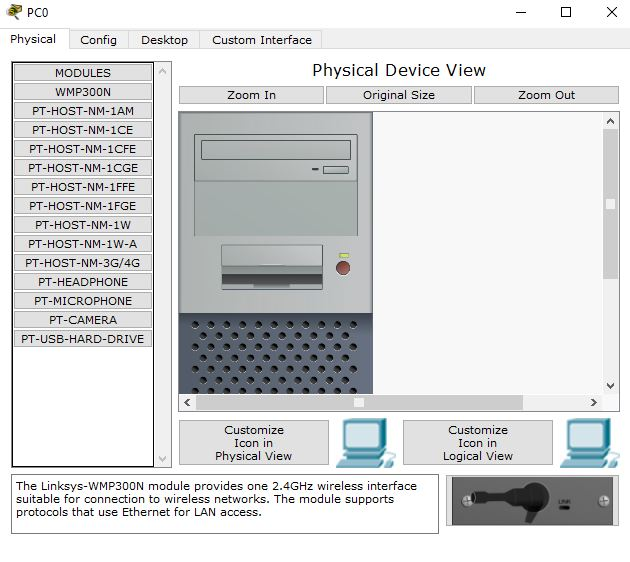
\includegraphics[width=0.6\linewidth]{images/07.routing-sicurezza/01.open-pc.jpg}
    \end{sfigure}
    \item Entrare nel Desktop del pc tramite il menu sovrastante\par
    \begin{sfigure}
        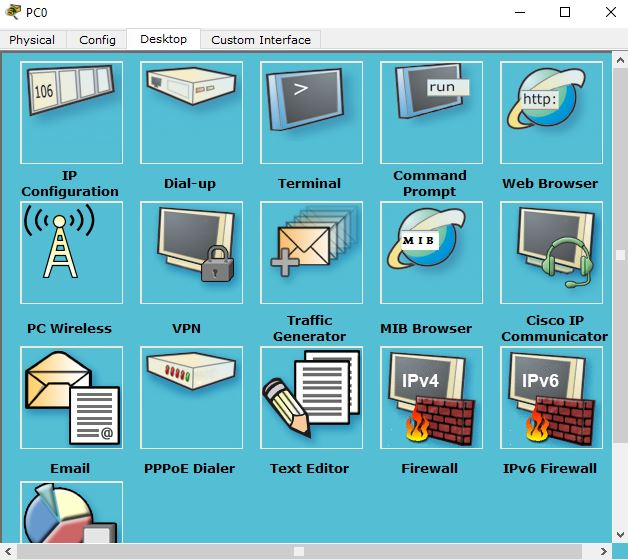
\includegraphics[width=0.6\linewidth]{images/07.routing-sicurezza/02.desktop-tab.jpg}
    \end{sfigure}
    \item Entrare nel menu della configurazione IP tramite l’icona presente nel desktop\par
    \begin{sfigure}
        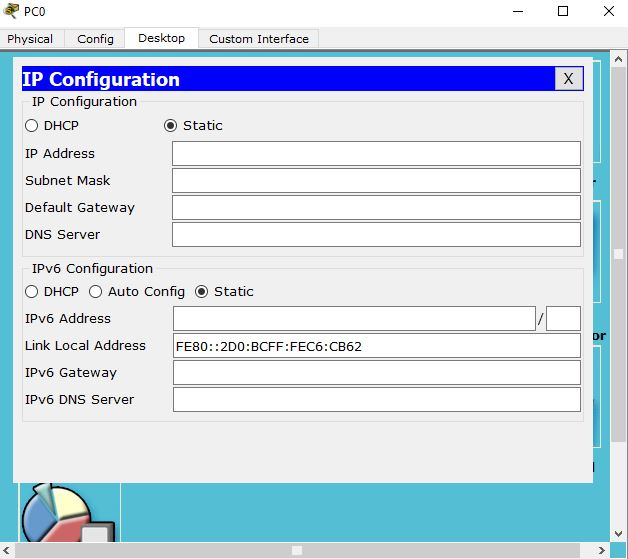
\includegraphics[width=0.6\linewidth]{images/07.routing-sicurezza/03.ip-config.jpg}
    \end{sfigure}
    \item In conclusione, inserire i dati riguardante gli indirizzi IP all’interno degli appositi come nell’esempio sotto riportato\par
    \begin{sfigure}
        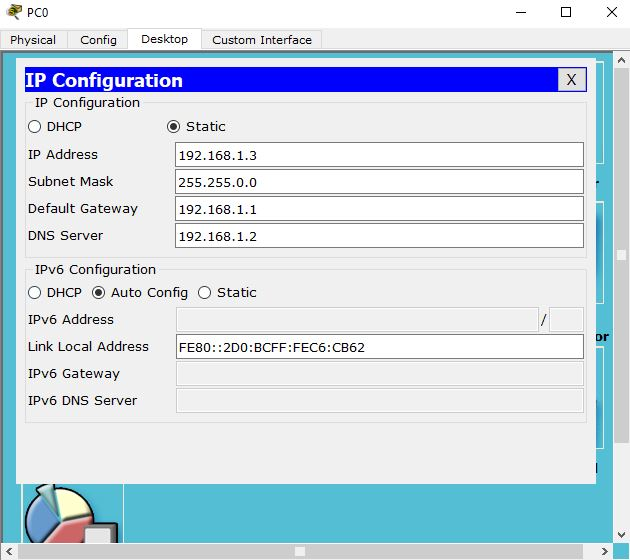
\includegraphics[width=0.6\linewidth]{images/07.routing-sicurezza/04.ip-config-complete.jpg}
    \end{sfigure}
\end{enumerate}

\subsubsection*{IP Route}
Il comando ip route è essenziale per la comunicazione tra reti a routing statico, dato che permette di creare rotte statiche e di conseguenza, instaurare il collegamento tra sottoreti. La sintassi del comando è molto semplice come vedremo a breve

Ecco come aggiungere una rotta tra router:

\begin{cmds}[Router]{Configuration mode}{cmd:ip-route-example}{Aggiungere una rotta statica nel router che indirizza i pacchetti destinati alla \textcolor{Highlight1}{rete specificata} verso l'\textcolor{Highlight2}{indirizzo IP o l'interfaccia} designata }
    \$ ip route \textcolor{Highlight1}{192.168.1.0 255.255.255.0} \textcolor{Highlight2}{172.16.100.1}
\end{cmds}

\subsection{VLAN}
Con il termine VLAN (Virtual Local Area Network) si intende la suddivisione di una rete locale, definita da uno switch, in più reti virtuali non comunicanti tra di loro ma appartenenti alla stessa infrastruttura fisica.

Per procedere alla suddivisione di una rete locale in più VLAN è necessario programmare lo switch a cui è associata la rete, quindi accedere alla console e digitare i seguenti comandi:

\begin{cmds}[Switch]{Configuration mode}{cmd:create-vlan}{Creare una VLAN in uno switch con \textcolor{Highlight1}{id} e \textcolor{Highlight2}{nome} arbitrario tuttavia la VLAN con ID 1 è utilizzata come default quindi convenzionalmente si utilizza la cifra delle decine (10, 20, ...)}
    \$ vlan \textcolor{Highlight1}{10}\\
    \$ name \textcolor{Highlight2}{sinistra}\\
    \$ vlan \textcolor{Highlight1}{20}\\
    \$ name \textcolor{Highlight2}{destra}
\end{cmds}

Una volta definite le VLAN si può procedere ad assegnare ad ogni rete virtuale le porte dello switch, suppondendo che lo switch abbia 24 porte in totali:

\begin{cmds}{Configuration mode}{cmd:setup-vlan-ports}{Configurazione delle porte dello switch modificando l'intero \textcolor{Highlight1}{range} di porte e assegnandole ad una \textcolor{Highlight2}{determinata VLAN}}
    \$ interface range \textcolor{Highlight1}{Fa 0/5-14}\\
    \$ switchport mode access\\
    \$ switchport access \textcolor{Highlight2}{vlan 10}\\
    \$ interface range \textcolor{Highlight1}{Fa 0/15-24}\\
    \$ switchport mode access\\
    \$ switchport access \textcolor{Highlight2}{vlan 20}
\end{cmds}

Un dettaglio importante di cui tenere conto quando si progettano le VLAN è quello di lasciare alcune porte non assegnate, così da poter definire eventuali porte di tronco. Una porta di tronco è una porta dello switch collegata ad un dispositivo esterno alle VLAN (come un router) e serve per permettere la comunicazione tra VLAN e i dispositivi collegati a quella porta.

Definizione di una porta di tronco:

\begin{cmds}[Switch]{Interfaccia esterna}{cmd:trunk-port}{Configurazione dell'interfaccia di tronco}
    \$ switchport mode trunk\\
    \$ switchport trunk allowed vlan
\end{cmds}

\subsection{VPN}
\subsection{Tunneling}
Le informazioni che vengono trasmesse tramite Internet, o tra due dispositivi digitali, necessitano di protocolli. Tali protocolli dividono il messaggio in diverse parti (in genere due), una contenente i dati effettivi che vengono trasmessi e l'altra contenente le informazioni relative alle regole di trasmissione. Per poter stabilire una connessione, entrambe le parti coinvolte devono comprendere e utilizzare lo stesso protocollo di comunicazione. Un protocollo di tunneling include nel proprio datagramma un altro pacchetto di dati completo che utilizza un protocollo di comunicazione diverso. In sostanza, crea un tunnel tra due punti di una rete che possono trasmettere tra loro qualsiasi tipo di dato in tutta sicurezza.

In genere, questi tipi di protocolli vengono utilizzati per inviare i dati di una rete privata tramite una rete pubblica, solitamente quando si crea una VPN (Virtual Private Network), ma possono essere utilizzati anche per aumentare la sicurezza dei dati non crittografati che vengono inviati tramite una rete pubblica. Sono disponibili diversi protocolli di tunneling alquanto diffusi, ad esempio Secure Shell (SSH), Point-to-Point Tunneling (PPTP) e IPsec, ognuno dei quali è stato progettato per uno scopo specifico.

Poiché i protocolli di tunneling nascondono nel proprio datagramma un pacchetto completo, potrebbero essere utilizzati in modo improprio. Il tunneling viene spesso utilizzato per bypassare firewall non sofisticati o non configurati in modo adeguato includendo protocolli bloccati nei protocolli che il firewall lascia passare. L'uso dei protocolli di tunneling rende, inoltre, difficile il completamento di attività quali il controllo dettagliato dei pacchetti, in cui l'infrastruttura di rete analizza il datagramma alla ricerca di dati sospetti, o il filtraggio dei dati in entrata/uscita, che esegue il test di integrità funzionale degli indirizzi di destinazione dei dati per evitare potenziali attacchi. Si registrano anche casi di malware trasmessi tramite la nuova tecnologia IPv6, che deve utilizzare il tunneling per la trasmissione verso o tramite dispositivi non compatibili.

In quanto potenziale minaccia, i protocolli di tunneling devono essere utilizzati solo da professionisti IT o di rete che possano garantire che i propri sistemi siano in grado di bloccare tunnel indesiderati e siano configurati in modo da poter applicare i protocolli di sicurezza ai dati inviati tramite un tunnel noto, analogamente ai dati inviati tramite una VPN.

\subsubsection{Vantaggi}
\begin{itemize}
    \item Permette ad un protocollo straniero di essere usato su una rete che non lo supporta; (Bypassare i blocchi geografici)
    \item Protegge dall'intercettazione dei dati; (connessione sicura)
    \item Bypassare i Firewall (es. Un firewall locale potrebbe essere, per esempio, quello di un’università che non consente di collegarsi a Netflix, o un firewall nel tuo posto di lavoro, che blocca determinati siti, come ad esempio YouTube. Connettendoti tramite una VPN, il problema non esiste più.)
    \item Nasconde l’indirizzo IP;
    \item I siti visitati vedranno solo la posizione del server VPN a cui sei connesso e non la posizione reale.
\end{itemize}

\subsubsection{Svantaggi}
\begin{itemize}
    \item Connessione internet lenta, poiché essa deve venire re-instradata e criptata tramite il server.
    \item Non supportato da tutti i dispositivi
\end{itemize}

\subsubsection{Componenti Cisco}

\subsubsection*{Network devices}
Per prima cosa \textbf{verificare che i router siano compatibili} con il protocollo IPv6.\\
Due router compatibili sono: 2811 e 2911

In questo progetto utilizzeremo: 2x Router 2911, Tunnel1 e Tunnel2

\begin{center}
    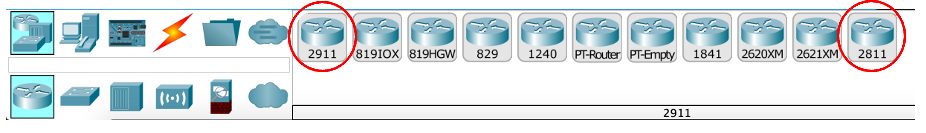
\includegraphics[width=\linewidth]{images/07.routing-sicurezza/tunneling/01.routers.png}
\end{center}

2x Switch 2950T-24 (Switch4 e Switch2)

\begin{center}
    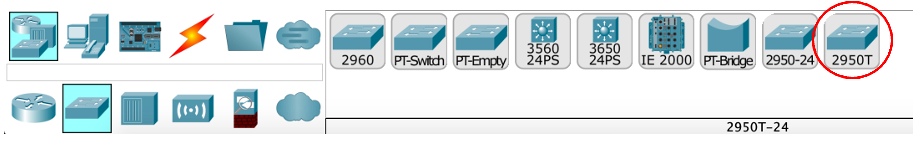
\includegraphics[width=\linewidth]{images/07.routing-sicurezza/tunneling/02.png}
\end{center}

\subsubsection*{End devices}
2x PC-PT (PC7 e PC8)

\begin{center}
    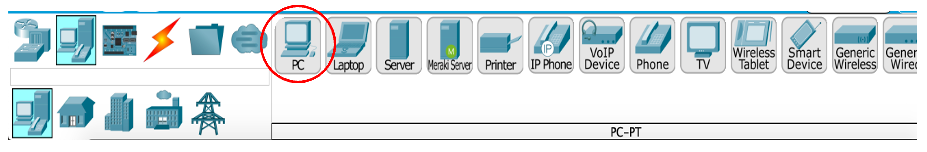
\includegraphics[width=\linewidth]{images/07.routing-sicurezza/tunneling/03.png}
\end{center}

\subsubsection*{Cavi}
Copper Cross-Over da Router0 e Router1 ai Router Tunnel1 e Tunnel2

\begin{center}
    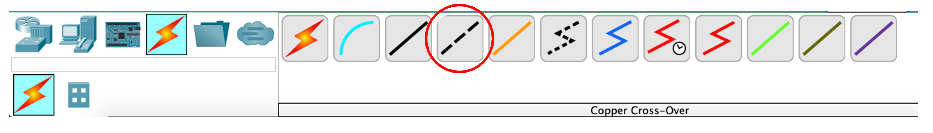
\includegraphics[width=\linewidth]{images/07.routing-sicurezza/tunneling/04.png}
\end{center}

\noindent Copper Straight-Through dai Router Tunnel1 e Tunnel2 agli Switch4 e Switch2 e dagli Switch4 e Switch2 ai PC7 e PC8

\begin{center}
    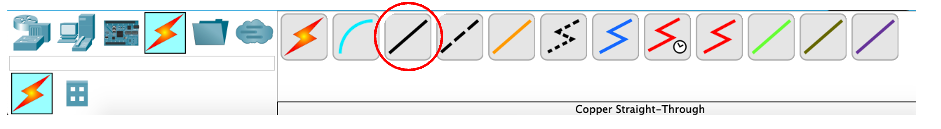
\includegraphics[width=\linewidth]{images/07.routing-sicurezza/tunneling/05.png}
\end{center}

\subsubsection*{Porte Router Tunnel1}

\begin{center}
    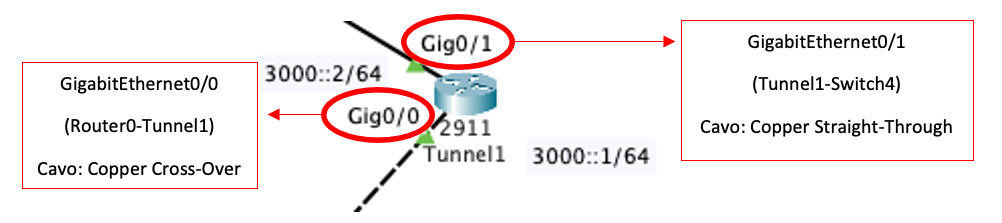
\includegraphics[width=\linewidth]{images/07.routing-sicurezza/tunneling/06.png}
\end{center}

\subsubsection*{Porte Router Tunnel2}

\begin{center}
    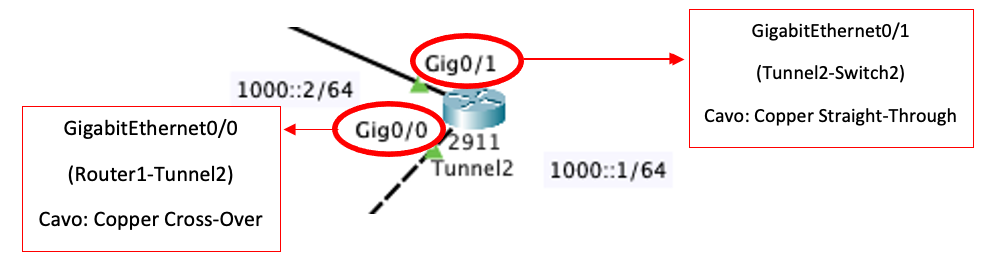
\includegraphics[width=\linewidth]{images/07.routing-sicurezza/tunneling/07.png}
\end{center}

\subsubsection*{Porte Switch4 e PC7:}

\begin{center}
    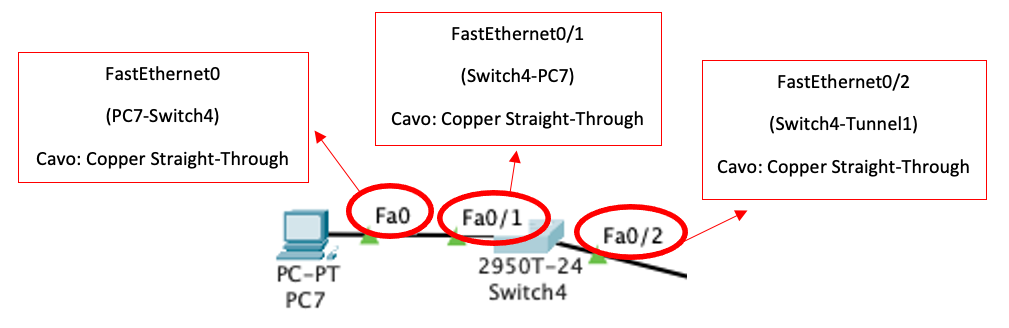
\includegraphics[width=\linewidth]{images/07.routing-sicurezza/tunneling/08.png}
\end{center}

\subsubsection*{Porte Switch2 e PC8:}

\begin{center}
    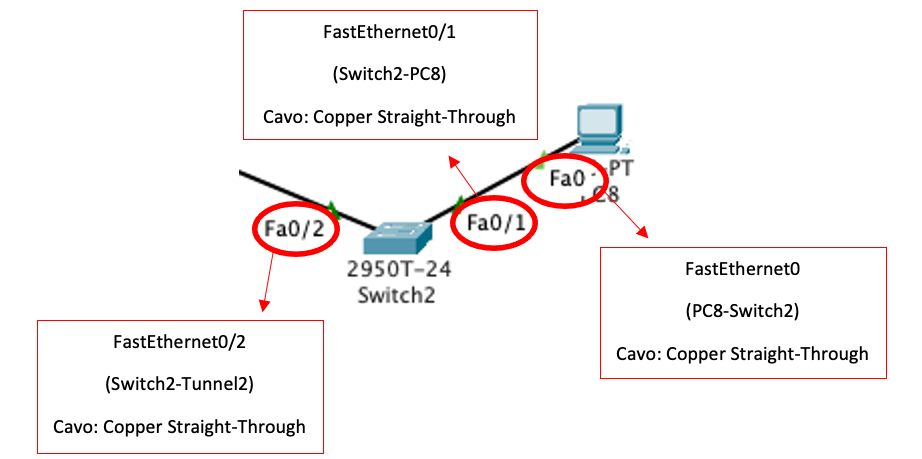
\includegraphics[width=\linewidth]{images/07.routing-sicurezza/tunneling/09.png}
\end{center}

\subsubsection{Realizzazione Tunneling}
Per poter effettuare la tecnica del tunneling sul programma Cisco Packet Tracer (in questo caso nella versione Student Version 6.2.0.0052) basterà seguire questi passaggi:

\begin{enumerate}
    \item Per prima cosa dobbiamo entrare nel Router “Tunnel2” del nostro progetto, recandoci nella sezione “CLI” di esso (Command Line Interface);\par
    \begin{center}
        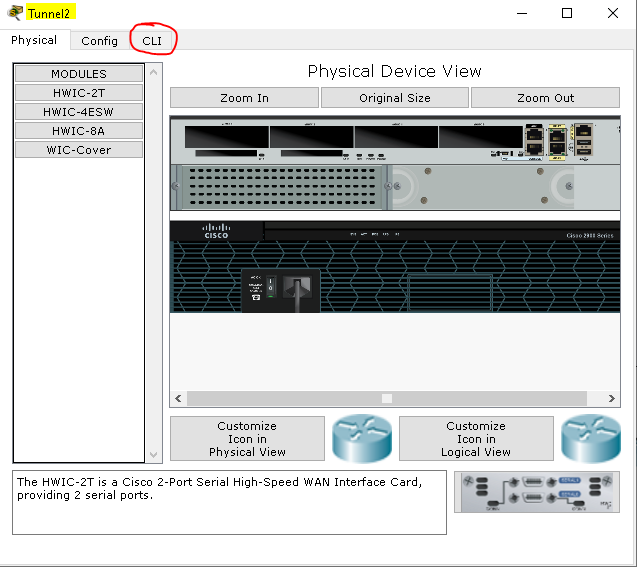
\includegraphics[width=\linewidth]{images/07.routing-sicurezza/tunneling/10.png}
    \end{center}
    \item A questo punto dovranno essere inseriti i seguenti comandi in questo ordine:\par
    \begin{cmds}{Configuration mode}{cmd:setup-tunneling-1}{Configurazione Tunneling}
        \$ ipv6 unicast-routing\\
        \$ interface tunnel 0\\
        \$ ipv6 address 2000::2/64\\
        \$ ipv6 rip 5info enable\\
        \$ tunnel source Gig0/0\\
        \$ tunnel destination 192.168.8.218/30\\
        \$ tunnel mode ipv6ip\\
        \$ no shutdown
    \end{cmds}
    \item Ora che il tunnel è stato impostato, configuriamo le porte che verranno utilizzate su questo router:\par
    \begin{cmds}{Configuration mode}{cmd:setup-tunneling-2}{Configuratione Porte}
        \$ interface Gig0/1\\
        \$ ipv6 enable\\
        \$ ipv6 address 1000::1/64\\
        \$ ipv6 rip 6bone enable\\
        \$ no shutdown\\
        \$ exit\\
        \$ interface Gig0/0\\
        \$ ip address 192.168.8.214 255.255.255.252\\
        \$ no shutdown
    \end{cmds}
    \item Configuriamo ora l’altro router (Tunnel1) incluso nel tunnel che stiamo creando;
    \item Ci rechiamo dunque anche in esso nell’interfaccia “CLI” e inseriamo i seguenti comandi:\par
    \begin{cmds}{Configuration mode}{cmd:setup-tunneling-3}{Configurazione Tunnel1 altro Router}
        \$ ipv6 unicast-routing\\
        \$ interface tunnel 0\\
        \$ ipv6 address 2000::1/64\\
        \$ ipv6 rip 6bone enable\\
        \$ tunnel source Gig0/0\\
        \$ tunnel destination 192.168.8.214/30\\
        \$ tunnel mode ipv6ip\\
        \$ no shutdown\\
        \$ interface Gig0/1\\
        \$ ipv6 enable\\
        \$ ipv6 address 3000::1/64\\
        \$ ipv6 rip 5info enable\\
        \$ no shutdown
    \end{cmds}
    \item A questo punto abbiamo bisogno di effettuare l’Ip Route nei due router per rendergli possibile l’instradamento delle informazioni attraverso il tunnel che stiamo creando;
    \item Accediamo dunque al router “Tunneling1” e sempre nella sezione “CLI” digitiamo I seguenti comandi:\par
    \begin{cmds}{Configuration mode}{cmd:setup-tunneling-4}{Configurazione Routes}
        \$ ip route 192.168.8.212 255.255.255.252 2000::2/64
    \end{cmds}
    \item Facciamo la stessa cosa con il router “Tunneling2”:\par
    \begin{cmds}{Configuration mode}{cmd:setup-tunneling-4}{Configurazione Routes}
        \$ ip route 192.168.8.216 255.255.255.252 2000::1/64
    \end{cmds}
    \item Ora avremmo così creato la seguente topologia:\par
    \begin{center}
        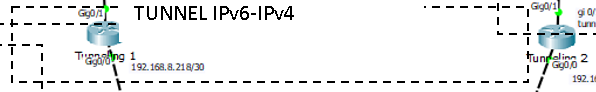
\includegraphics[width=\linewidth]{images/07.routing-sicurezza/tunneling/11.png}
    \end{center}
\end{enumerate}
